\documentclass[12pt,letterpaper]{exam}
\usepackage[lmargin=1in,rmargin=1in,tmargin=1in,bmargin=1in]{geometry}
\usepackage{../style/exams}

% -------------------
% Course & Exam Information
% -------------------
\newcommand{\course}{MATH 111I: Exam 2}
\newcommand{\term}{Spring --- 2025}
\newcommand{\examdate}{03/27/2025}
\newcommand{\timelimit}{75 Minutes}

\setbool{hideans}{false} % Student: True; Instructor: False

% -------------------
% Content
% -------------------
\begin{document}

\examtitle
\instructions{Write your name on the appropriate line on the exam cover sheet. This exam contains \numpages\ pages (including this cover page) and \numquestions\ questions. Check that you have every page of the exam. Answer the questions in the spaces provided on the question sheets. Be sure to answer every part of each question and show all your work. If you run out of room for an answer, continue on the back of the page --- being sure to indicate the problem number.} 
\scores
\bottomline
\newpage


% -------------------
% Questions
% -------------------
\begin{questions}

% Question 1
\newpage
\question[8] Showing all your work, factor the following as must as possible: \par\vspace{0.3cm}
	\begin{parts}
	\part $x^2 + 8x - 48$ \pspace
	\sol{We find factors of $1 \cdot -48= -48$ that add to $8$. Because $-48 < 0$, the factors must have opposite signs.
	\begin{table}[!ht]
	\centering
	\wsol{\underline{\bfseries $\mathbf{-48}$}} \pvspace{0.2cm}
	\begin{tabular}{rr}
	\wsol{$1 \cdot -48$} & \wsol{$-47$} \\
	\wsol{$-1 \cdot 48$} & \wsol{$47$} \\
	\wsol{$2 \cdot -24$} & \wsol{$-22$} \\
	\wsol{$-2 \cdot 24$} & \wsol{$22$} \\
	\wsol{$3 \cdot -16$} & \wsol{$-13$} \\
	\wsol{$-3 \cdot 16$} & \wsol{$13$} \\
	\wsol{$4 \cdot -12$} & \wsol{$-8$} \\
	\wsol{\underline{$\mathbf{-4 \cdot 12}$}} & \wsol{\underline{$\mathbf{8}$}} \\
	\wsol{$6 \cdot -8$} & \wsol{$-2$} \\
	\wsol{$-6 \cdot 8$} & \wsol{$2$}
	\end{tabular}
	\end{table} \par
	Therefore, we have\dots
		\[
		x^2 + 8x - 48= \boxed{(x - 4)(x + 12)}
		\] \vfill
	}

	\part $4x^2 - 9$ \pspace
	\sol{Recall that a difference of perfect square, $a^2 - b^2$, factors as $(a - b)(a + b)$. We have $a= 2x$ (so that $a^2= (2x)^2= 4x^2$) and $b= 3$ (so that $b^2= 3^2= 9$). Therefore, we have\dots
		\[
		4x^2 - 9= \boxed{(2x - 3)(2x + 3)}
		\] \par\vspace{4cm}\vfill
	}
	\end{parts}



% Question 2
\newpage
\question[8] Showing all your work, solve the following equation:
	\[
	x(x + 1)= 20
	\]

\sol{{\itshape\bfseries Solution.} We have\dots
	\[
	\begin{gathered}
	x(x + 1)= 20 \\[0.3cm]
	x^2 + x= 20 \\[0.3cm]
	x^2 + x - 20= 0 \\[0.3cm]
	(x + 5)(x - 4)= 0
	\end{gathered}
	\] \pspace
But then either $x + 5= 0$, which implies that $x= -5$, or $x - 4= 0$, which implies that $x= 4$. Therefore, we have\dots \par\vspace{0.2cm}
	\[
	\boxed{x= -5, \, 4}
	\] \vfill
}



% Question 3
\question[8] Showing all your work, solve the following equation:
	\[
	x^2 + 24= 10x
	\]

\sol{{\itshape\bfseries Solution.} We have\dots
	\[
	\begin{gathered}
	x^2 + 24= 10x \\[0.3cm]
	x^2 - 10x + 24= 0 \\[0.3cm]
	(x - 4)(x - 6)= 0
	\end{gathered}
	\] \pspace
But then either $x - 4= 0$, which implies that $x= 4$, or $x - 6= 0$, which implies that $x= 6$. Therefore, we have\dots \par\vspace{0.2cm}
	\[
	\boxed{x= 4, \, 6}
	\] \vfill
}



% Question 4
\newpage
\question[10] Consider the quadratic function $f(x)= 10 - (x + 6)^2$.
	\begin{parts}
	% (a)
	\part What is the vertex for $f(x)$? \pspace
	\sol{The $x$-coordinate of the vertex makes the square term $0$. Clearly, the $x$-coordinate of the vertex is $x= -6$. The $y$-coordinate of the vertex is what remains once the square term is $0$, which here is $10$. Therefore, the vertex is $(-6, 10)$.} \pspace \vfill
	% (b)
	\part What is the domain of $f(x)$? \pspace
	\sol{Because $f(x)$ is a polynomial, the domain of $f(x)$ is all real numbers, i.e. the domain of $f(x)$ is $(-\infty, \infty)$. Equivalently, one can say that the domain of $f(x)$ is $\mathbb{R}$.} \pspace \vfill
	% (c)
	\part Is $f(x)$ concave up or concave down? Justify your answer. \pspace
	\sol{Writing $f(x)$ as $-(x + 6)^2 + 10$, we can see that $a= -1$. Alternatively, we have $f(x)= 10 - (x + 6)(x + 6)= 10 - (x^2 + 6x + 6x + 36)= 10 - (x^2 + 12x - 36)= 10 - x^2 - 12x - 36= -x^2 - 12x - 26$. In any case, we have $a= -1 < 0$. Therefore, $f(x)$ opens downwards; that is, $f(x)$ is concave down.} \pspace \vfill
	% (d)
	\part Does $f(x)$ have a maximum value or a minimum value? Explain. \pspace
	\sol{Because $f(x)$ opens downwards, we know that $f(x)$ has a `highest point'---the vertex. Therefore, it must be that $f(x)$ has a maximum value. However, there is no minimum value for $f(x)$.} \pspace \vfill
	% (e)
	\part Find the maximum or minimum value for $f(x)$---whichever exists. \pspace
	\sol{We know from the previous part that $f(x)$ has a maximum value. We know that the `highest point' on $f(x)$ is the vertex. The $y$-value of the vertex is the `output at this highest point.' We know from (a) that the vertex is $(-6, 10)$. Therefore, the maximum value for $f(x)$ is $10$.} \pspace \vfill
	% (f)
	\part What is the range of $f(x)$? \pspace
	\sol{We know from (d) and (e) that $f(x)$ has a maximum value of $10$. We know also from (c) that $f(x)$ opens downwards. Therefore, it must be that $f(x)$ `takes on' every value $10$ or less. Therefore, the range of $f(x)$ is $(-\infty, 10]$.} \pspace \vfill
	\end{parts}



% Question 5
\newpage
\question[8] Showing all your work, solve the following equation:
	\[
	x= \sqrt{x} + 2
	\] \pspace

\sol{{\itshape\bfseries Solution.} We have\dots
	\[
	\begin{gathered}
	x= \sqrt{x} + 2 \\
	x - 2= \sqrt{x} \\
	(x - 2)^2= (\sqrt{x})^2 \\
	x^2 - 2x - 2x + 4= x \\
	x^2 - 4x + 4= x \\
	x^2 - 5x + 4= 0 \\
	(x - 1)(x - 4)= 0 
	\end{gathered}
	\] \pspace
But then either $x - 1= 0$, which implies that $x= 1$, or $x - 4= 0$, which implies that $x= 4$. Alternatively, suppose we write $y= \sqrt{x}$, so that $y^2= (\sqrt{x})^2= x$. But then\dots
	\[
	\begin{gathered}
	x= \sqrt{x} + 2 \\
	y^2= y + 2 \\
	y^2 - y - 2= 0 \\
	(y - 2)(y + 1)= 0 
	\end{gathered}
	\]
But then either $y - 2= 0$, so that $y= 2$. But then $\sqrt{x}= 2$, so that $x= \sqrt{x}^2= 2^2= 4$. Or we know that $y + 1= 0$, so that $y= -1$. But then $\sqrt{x}= -1$, so that $x= \sqrt{x}^2= (-1)^2= 1$. \pspace

However, not both of these are solutions. We can verify that $x= 4$ is a solution:
	\[
	\begin{gathered}
	x= \sqrt{x} + 2 \\
	4\stackrel{?}{=} \sqrt{4} + 2 \\
	4\stackrel{?}{=} 2 + 2 \\
	4= 4
	\end{gathered}
	\]
However, $x= 1$ is not a solution (it is an extraneous solution):
	\[
	\begin{gathered}
	x= \sqrt{x} + 2 \\
	1\stackrel{?}{=} \sqrt{1} + 2 \\
	1\stackrel{?}{=} 1 + 2 \\
	1 \neq 3
	\end{gathered}
	\]
Therefore, the only solution is $x= 4$:
	\[
	\boxed{x= 4}
	\]
}



% Question 6
\newpage
\question[8] Showing all your work, find the vertex form of $x^2 - 12x + 44$. \pspace

\sol{{\itshape\bfseries Solution.} The `middle' term is $-12$. Taking half of this, we have $\frac{-12}{2}= -6$. Squaring this value, we have $(-6)^2= 36$. But then by completing the square, we have\dots
	\[
	\begin{gathered}
	x^2 - 12x + 44 \\[0.3cm]
	x^2 - 12x + 36 - 36 + 44 \\[0.3cm]
	(x^2 - 12x + 36) + (-36 + 44) \\[0.3cm]
	\boxed{(x - 6)^2 + 8}
	\end{gathered}
	\] \par\vspace{1cm}

Alternatively, using the `Evaluation Method', we know the $x$-coordinate of the vertex is $x= -\frac{b}{2a}$. We know that $a= 1$, $b= -12$, and $c= 44$. Therefore, the $x$-coordinate of the vertex is\dots
	\[
	x= -\dfrac{b}{2a}= -\dfrac{-12}{2(1)}= -\dfrac{-12}{2}= -(-6)= 6
	\] \pspace
Letting $f(x)= x^2 - 12x + 44$, we know the $y$-coordinate of the vertex is\dots
	\[
	f(6)= 6^2 - 12(6) + 44= 36 - 72 + 44= -36 + 44= 8
	\] \pspace
We know that the vertex form is $y= a(x - P)^2 + Q$, where the vertex is $(P, Q)$ and $a$ is the $a$-value from the standard form. The vertex is $(P, Q)= (6, 8)$. Therefore, the vertex form is\dots
	\[
	1(x - 6)^2 + 8= \boxed{(x - 6)^2 + 8}
	\]
}



% Question 7
\newpage
\question[8] Showing all your work, factor the following as must as possible: \par\vspace{0.3cm}
	\begin{parts}
	\part $2x^2 - 15x - 8$ \pspace
	\sol{We find factors of $2 \cdot -8= -16$ that add to $-15$. Because $-16 < 0$, the factors must have opposite signs.
	\begin{table}[!ht]
	\centering
	\wsol{\underline{\bfseries $\mathbf{-16}$}} \pvspace{0.2cm}
	\begin{tabular}{rr}
	\wsol{\underline{$\mathbf{1 \cdot -16}$}} & \wsol{\underline{$\mathbf{-15}$}} \\
	\wsol{$-1 \cdot 16$} & \wsol{$15$} \\
	\wsol{$2 \cdot -8$} & \wsol{$-6$} \\
	\wsol{$-2 \cdot 8$} & \wsol{$6$} \\
	\wsol{$4 \cdot -4$} & \wsol{$0$} \\
	\wsol{$-4 \cdot 4$} & \wsol{$0$}
	\end{tabular}
	\end{table} \par
	Therefore, we have\dots
		\[
		2x^2 - 15x - 8= 2x^2 + x - 16x - 8= x(2x + 1) - 8(2x + 1)= \boxed{(2x + 1)(x - 8)}
		\] \vfill
	}

	\part $x^3 - 4x^2 + 3x$ \pspace
	\sol{First, we factor out an $x$: $x^3 - 4x^2 + 3x= x(x^2  - 4x + 3)$. We then need to factor $x^2  - 4x + 3$. We find factors of $3$ that add to $-4$. Because $3 > 0$, the factors must have the same signs.
	\begin{table}[!ht]
	\centering
	\wsol{\underline{\bfseries $\mathbf{3}$}} \pvspace{0.2cm}
	\begin{tabular}{rr}
	\wsol{$1 \cdot 3$} & \wsol{$4$} \\
	\wsol{\underline{$\mathbf{-1 \cdot -3}$}} & \wsol{\underline{$\mathbf{-4}$}} 
	\end{tabular}
	\end{table} \par
	Therefore, we have\dots
		\[
		x^3 - 4x^2 + 3x= x(x^2  - 4x + 3)= \boxed{x(x - 1)(x - 3)}
		\] \vfill
	}
	\end{parts}



% Question 8
\newpage
\question Consider the quadratic function $45x^2 - 148x + 96$.
	\begin{parts}
	% (a)
	\part[3] Use the discriminant of the given quadratic to explain why it factors \textit{without} explicitly factoring it. \pspace
	\sol{\small We know the discriminant of a quadratic function $ax^2 + bx + c$ is $D= b^2 - 4ac$. We have $a= 45$, $b= -148$, and $c= 96$. Therefore, the discriminant of this quadratic function is\dots
		\[
		D= b^2 - 4ac= (-148)^2 - 4(45)96= 21904 - 17280= 4624
		\]
	We know that the quadratic function factors if the discriminant is a perfect square. We can see that $D$ is a perfect square because $\sqrt{D}= \sqrt{4624}= 68$, i.e. $68^2= 4624$. Therefore, $45x^2 - 148x + 96$ factors.
	} 
	% (b)
	\part[4] Use the quadratic formula to find the $x$-intercepts of the given quadratic. \pspace
	\sol{We have\dots
		\[
		\begin{aligned}
		x&= \dfrac{-b \pm \sqrt{b^2 - 4ac}}{2a} \\
		&= \dfrac{-(-148) \pm \sqrt{D}}{2(45)} \\
		&= \dfrac{148 \pm \sqrt{4624}}{90} \\
		&= \dfrac{148 \pm 68}{90}
		\end{aligned}
		\] \pspace
	Therefore, the $x$-intercepts are $x= \dfrac{148 - 68}{90}= \dfrac{80}{90}= \dfrac{8}{9}$ and $x=\dfrac{148 + 68}{90}= \dfrac{216}{90}= \dfrac{12}{5}$\,, i.e. $\boxed{x= \dfrac{8}{9}, \, \dfrac{12}{5}}$\,. \par
	} \vfill
	% (c)
	\part[3] Use the previous part to factor the given quadratic. \pspace
	\sol{\small We `unsolve' for $x$:
		\[
		\begin{aligned}
		x&= \dfrac{8}{9} &\hspace{3cm} x&= \dfrac{12}{5} \\
		9x&= 8 & 5x&= 12 \\
		9x - 8&= 0 & 5x - 12&= 0
		\end{aligned}
		\]
	Therefore, $9x - 8$ and $5x - 12$ are factors of $45x^2 - 148x + 96$.  Because $9 \cdot 5= 45= a$, we know that\dots
		\[
		45x^2 - 148x + 96= \boxed{(9x - 8)(5x - 12)}
		\]
	}
	\end{parts}



% Question 9
\newpage
\question[8] For each of the given functions below, find functions $f(x)$ and $g(x)$ so that the given function can be written as $f \big( g(x) \big)$. \par\vspace{0.3cm}
	\begin{parts}
	\part $(x - 5)^3$ \pspace
	\sol{There are infinitely many possible answers. The `most obvious' choice is\dots
		\[
		\boxed{
		\begin{gathered}
		f(x)= x^3 \\[0.3cm]
		g(x)= x - 5
		\end{gathered}
		}
		\] \pspace
	We can verify this:
		\[
		f \big( g(x) \big)= f(x - 5)= (x - 5)^3
		\]
	} \vfill
	
	\part $\dfrac{1}{2x + 9}$ \pspace
	\sol{There are infinitely many possible answers. The `most obvious' choice is\dots
		\[
		\boxed{
		\begin{gathered}
		f(x)= \dfrac{1}{x} \\
		g(x)= 2x + 9
		\end{gathered}
		}
		\] \pspace
	We can verify this:
		\[
		f \big( g(x) \big)= f(2x + 9)= \dfrac{1}{2x + 9}
		\]
	} \vfill
	\end{parts}



% Question 10
\newpage
\question[9] Showing any necessary work, find the domain of each of the following functions: \par\vspace{0.3cm}
	\begin{parts}
	% (a)
	\part $x^3 - 5x + 12$ \pspace
	\sol{Because $x^3 - 5x + 12$ is a polynomial, the domain is all real numbers, i.e. the domain is $(-\infty, \infty)$. Alternatively, the domain is the set of all real numbers, $\mathbb{R}$.} \par\vspace{1cm} \vfill
	% (b)
	\part $\sqrt{x - 8}$ \pspace
	\sol{We know that $\sqrt{\Box{\phantom{x}}\!\!\!}$ is defined only if $\Box{\phantom{x}} \!\!\!\geq 0$. But then we need\dots
		\[
		\begin{gathered}
		x - 8 \geq 0 \\[0.3cm]
		x \geq 8
		\end{gathered}
		\] \pspace
	Therefore, the domain of $\sqrt{x - 8}$ is $\boxed{x \geq 8}$\,, i.e. the domain is $\boxed{[8, \infty)}$\,.
	} \vfill
	% (c)
	\part $\dfrac{1}{x + 5}$ \pspace
	\sol{\par We know that $\dfrac{1}{\Box{\phantom{x}}}$ is defined only if $\Box{\phantom{x}} \neq 0$. But then we need\dots
		\[
		\begin{gathered}
		x + 5 \neq 0 \\[0.3cm]
		x \neq -5
		\end{gathered}
		\] \pspace
	Therefore, the domain of $\dfrac{1}{x + 5}$ is $\boxed{\text{all real numbers except $x= -5$}}$\,, i.e. the domain is $(-\infty, -5) \cup (-5, \infty)$. Alternatively, the domain is $\mathbb{R} \setminus \{ -5 \}$.
	} \vfill
	\end{parts}



% Question 11
\newpage
\question[8] Three parts are given below. {\bfseries Choose any \underline{two} parts and complete these parts---showing all your work.} Cross out the part that you \textit{do not} want graded.
	\begin{enumerate}[(a)]
	% (a)
	\item Compared to the graph of $f(x)$, describe the graph of $y= -6 f(x + 5)$ in terms of $f(x)$. \pspace
	\sol{The graph of $y$ is the graph of $f(x)$ shifted 5 units to the left, scaled (stretched) by a factor 6 in the $y$-direction, and then reflected across the $x$-axis.} \vfill
	% (b)
	\item Find the function whose graph is the graph of a function $f(x)$ reflected through the $y$-axis, then shifted 2 units to the left, and then finally shifted 3 units down. \pspace
	\sol{The graph of $f(x)$ reflected through the $y$-axis is the graph of $f(-x)$. Shifting this 2 units to the left, we have $f(-x + 2)$. Finally, shifting this 3 units down, we have $f(-x + 2) - 3$. Therefore, the function is\dots
		\[
		\boxed{f(-x + 2) - 3}
		\]
	} \pspace
	% (c)
	\item The graph of $f(x)$ is shown below in black (the \textit{very} thick function). Determine what the function plotted in red is in terms of $f(x)$.
	\[
	\fbox{
	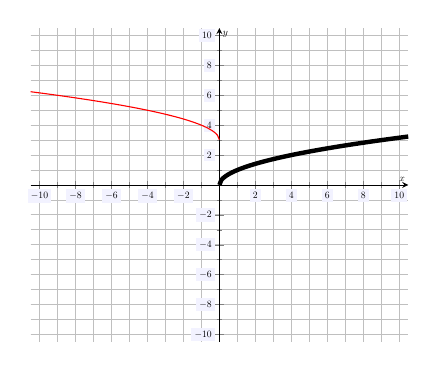
\begin{tikzpicture}[scale=0.7,every node/.style={scale=0.5}]
	\begin{axis}[
	grid=both,
	axis lines=middle,
	ticklabel style={fill=blue!5!white},
	xmin= -10.5, xmax=10.5,
	ymin= -10.5, ymax=10.5,
	xtick={-10,-8,...,10},
	ytick={-10,-8,...,10},
	minor tick = {-10,-9,...,10},
	xlabel=\(x\),ylabel=\(y\),
	]
	\addplot[line width=0.08cm, domain= 0:10.5, samples=100] ({x},{sqrt(x)});
	\addplot[line width=0.02cm, domain= -10.5:0, samples=100,red] ({x},{sqrt(-x) + 3});
	\end{axis}
	\end{tikzpicture}
	}
	\] 
	\sol{We can see that the graph of the red function is the graph of the black function, $f(x)$, reflected across the $y$-axis and then shifted 3 upwards. The function whose graph is the graph of $f(x)$ reflected across the $y$-axis is $f(-x)$. Shifting this 3 units upwards, we have $f(-x) + 3$. Therefore, the red function is given by\dots
		\[
		\boxed{f(-x) + 3}
		\]
	} \vfill
	\end{enumerate}



% Question 12
\newpage
\question[7] Let $f(x)$ be the function $f(x)= 3x - 7$.
	\begin{parts}
	% (a)
	\part The graph of $f(x)$ is shown below.
            	\[
            	\fbox{
            	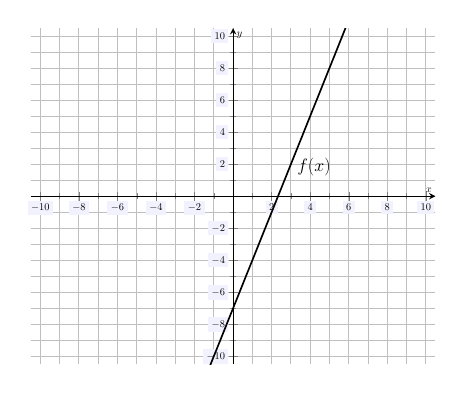
\begin{tikzpicture}[scale=0.75,every node/.style={scale=0.5}]
            	\begin{axis}[
            	grid=both,
            	axis lines=middle,
            	ticklabel style= {fill= blue!5!white},
            	xmin= -10.5, xmax=10.5,
            	ymin= -10.5, ymax=10.5,
            	xtick= {-10,-8,...,10},
            	ytick= {-10,-8,...,10},
            	minor tick = {-10,-9,...,10},
            	xlabel= \(x\), ylabel= \(y\)
            	]
            	\addplot[thick, samples=150, smooth, domain= -10.5:10.5] {3*x - 7};    
		\node at (4.2,1.8) {\LARGE$f(x)$};
            	\end{axis}
            	\end{tikzpicture}
            	}
            	\]
	Explain why the function $f(x)$ has an inverse, i.e. explain why $f^{-1}(x)$ exists. \pspace
	\sol{We know that the function $f(x)$ has an inverse, i.e. $f^{-1}(x)$ exists, because $f(x)$ passes the horizontal line test; that is, every horizontal line intersects the graph of $f(x)$ at most once.} \par\vspace{2cm}
	% (b)
	\part Showing all your work, find $f^{-1}(x)$. \pspace
	\sol{We write $y= 3x - 7$. To find $f^{-1}(x)$, we interchange the roles of $x$ and $y$, and then we solve for $y$. Interchanging the roles of $x$ and $y$, we have $x= 3y - 7$. We now solve for $y$:
		\[
		\begin{gathered}
		x= 3y - 7 \\[0.3cm]
		x + 7= 3y \\[0.3cm]
		\dfrac{x + 7}{3}= y 
		\end{gathered}
		\]
	Therefore, we have\dots
		\[
		\boxed{f^{-1}(x)= \dfrac{x + 7}{3}}
		\]
	}
	\end{parts}

\end{questions}
\end{document}